\begin{figure}[tbh]
		\centering
		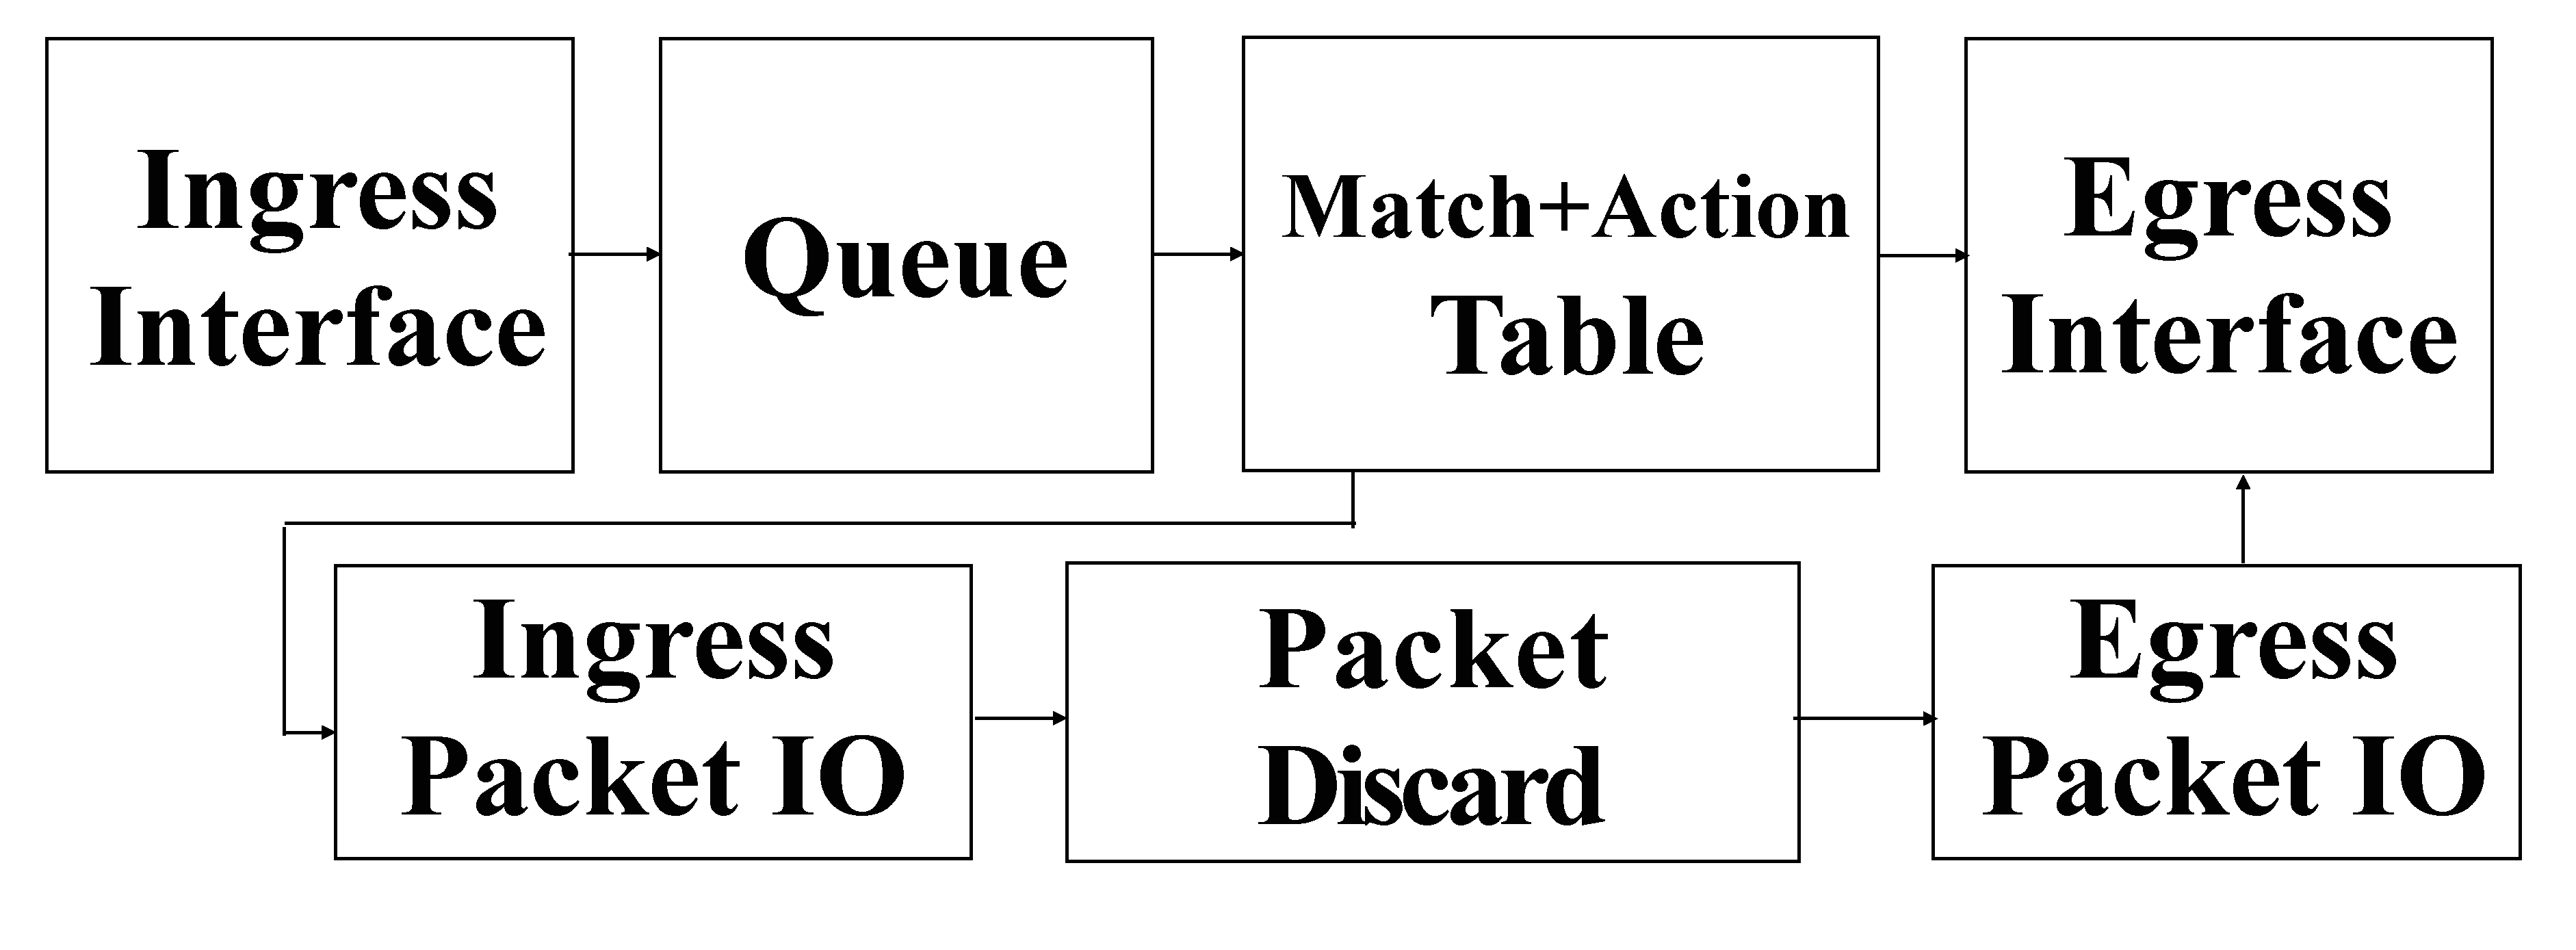
\includegraphics[width=.24\textwidth]{fig/MANE_1.eps}
		\caption{Packet processing in a P4-based MANE.}
		\label{MANE}
\end{figure}

\section{Media-Aware Network Element} \label{sec:mane}
\begin{comment}
{\em We show how to intelligently drop scalable video
packets to retain streamed video quality, when bandwidth is insufficient and
dynamic.} We consider three {\em packet discarding logics}: (i) tail, (ii)
enhancement-layer (EL), and (iii) rate-distortion optimized (RDO). Tail always
drops the last packet in the queue, while EL only drops the enhancement-layer
packets when needed. The advantage of tail logic is simplicity, while EL logic
ensures the decodability of received videos. RDO logic is more comprehensive,
as it takes the nonlinear nature between distortion and bitrate into
considerations. By dropping the packets with the least distortion and bitrate
ratio, RDO logic aims to minimize the negative impacts of dropping packets on
video quality.



We have implemented a MANE in P4 programming language~\cite{BDGI+14}. Fig.~\ref{MANE} shows
how the P4-based MANE processes the packets. First, we define the header formats
and parsers, which allow us to understand the structure of individual packets.
We use the information in headers to check if packets are valid.
Next, we define tables to describe how the header
fields should be matched in the match+action stage.  The control program pushes
the packets into one of the queues based on their header fields.  It starts to
throttle the ingress packets when the queue occupancy exceeds a
admin-specified threshold. More specifically, the {\em packet discard logic} picks and
drops some packets, in order to maintain high overall video streaming quality; 
other packets are forwarded.

% Bear, may be reused later
\begin{comment}
Programming Protocol Independent Packet Processors (P4) Language is a high-level language for constructing a packet-control system on a specific switch. It will first define parser information, control program, and flow table. Next, it defines actual packet parser, ingress control, egress control. The are differences between P4 and traditional SDN,  SDN controller can only process traditional packets but P4 can define our own packet format and decide what action should be made.

\begin{figure}[h]
		\centering
		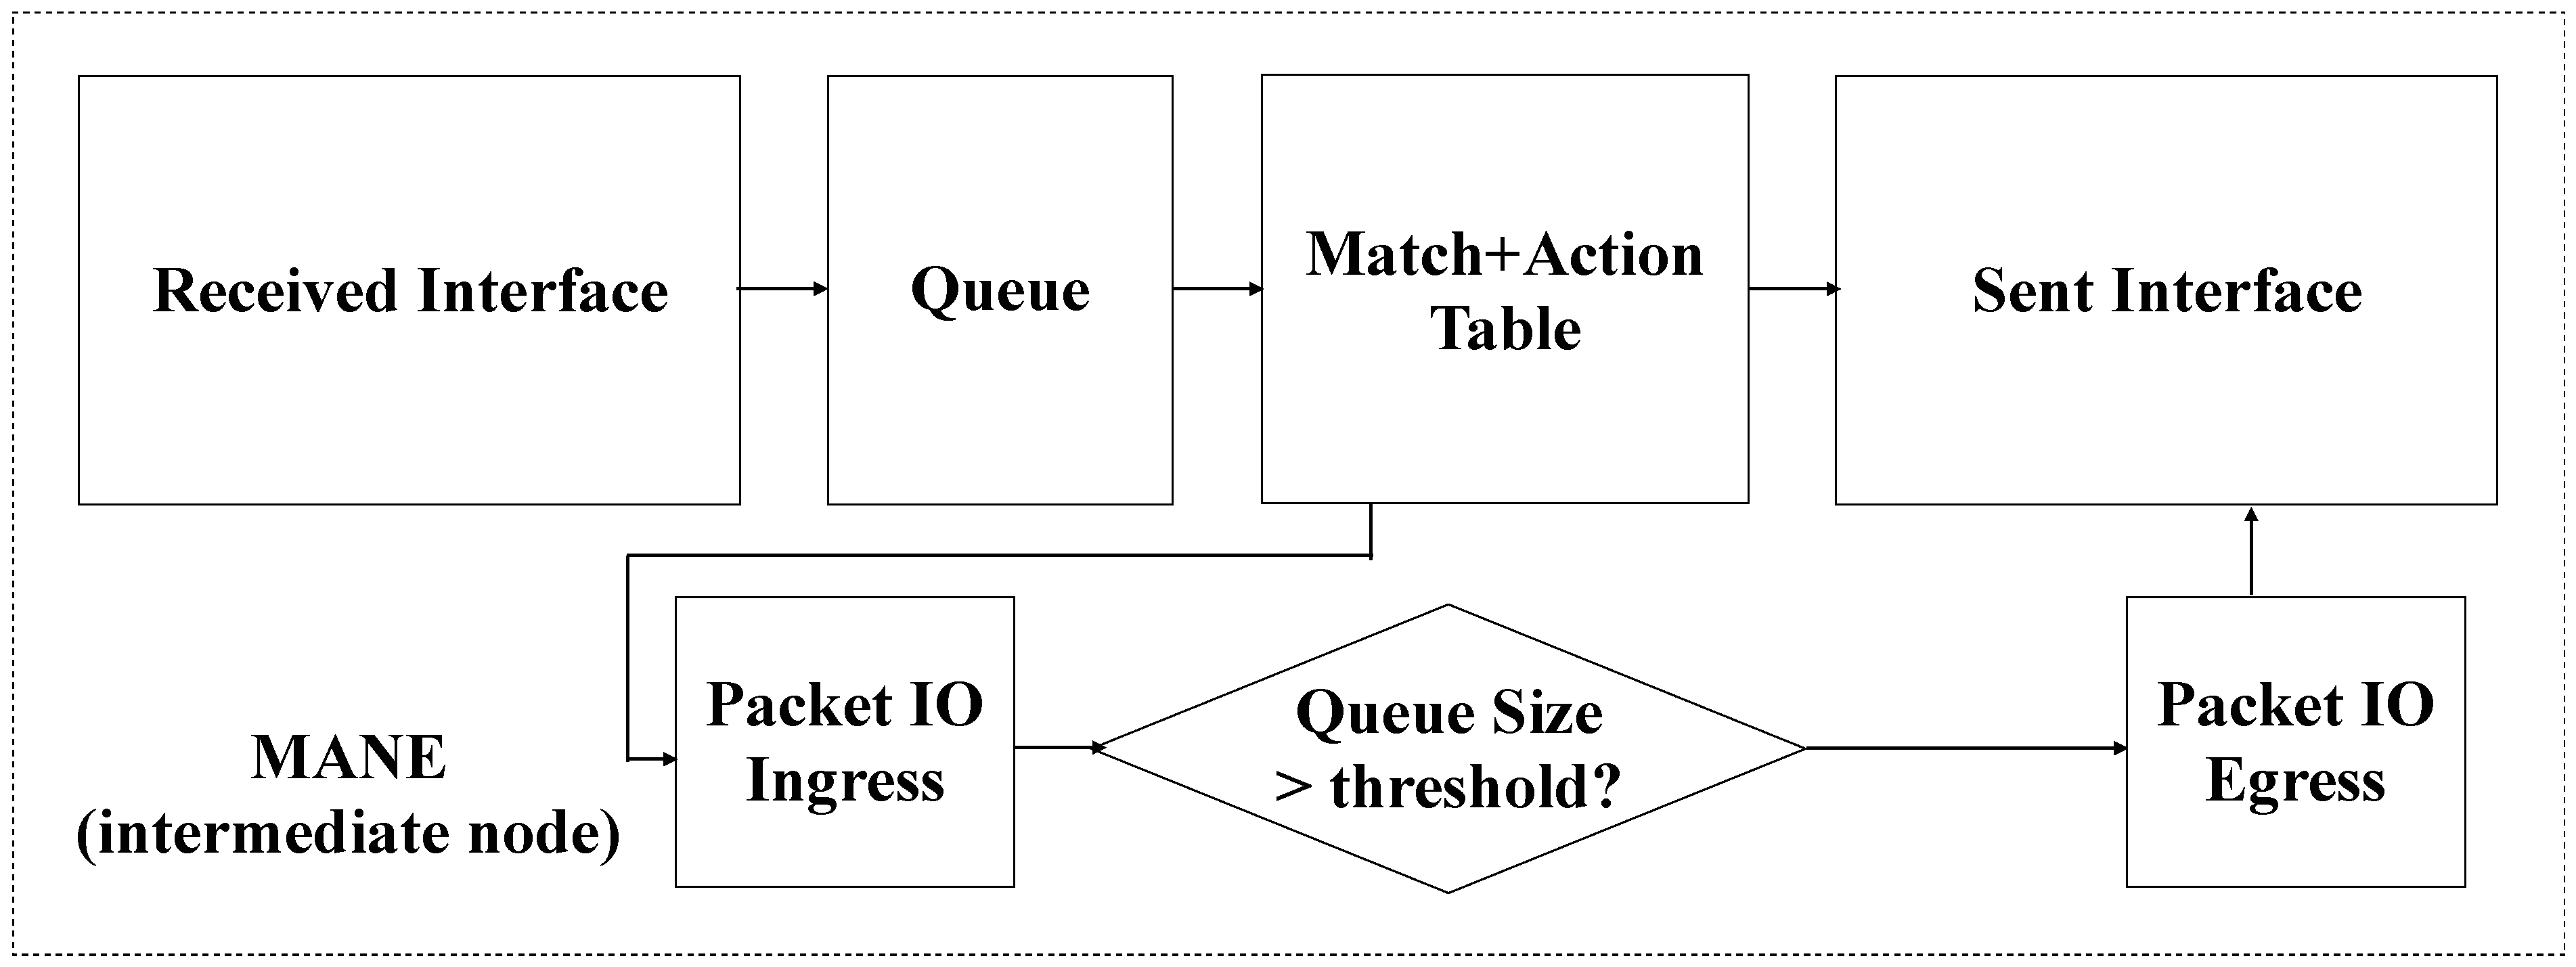
\includegraphics[width=5cm]{fig/network.eps}
		\caption{MANE Structure}
		\label{scenario_1}
\end{figure}

Layered video coding helps to supply multiple streams to meet the requirements of heterogeneous network environment. Scalable video coding(SVC) is a extension of traditional H.264/MPEG-4 AVC. It provides three mainly characteristic, temporal scalability, spatial scalabilility and SNR scalability. With these characteristics, SVC video transmission could be more adaptable in variety QoS demands. 

Media Aware Network Element(MANE) is an intermediate node between server and client. The MANE managers the SVC packets in the middle of the network. In this paper, our goal is to implement a P4 switch to act as a MANE. We define the packet format and how to handle packets in P4 switch. Next, we drop some of these packets if our queue is growing bigger and bigger. In scalable video steaming,the whole frame cannot be decode if the base layer is dropped. So this paper wants to keep more base layers as possible. However, we should maintain the video quality simultaneously. There are three algorithms to be considered.
\begin{itemize}
\item Tail drop
\item Base Only
\item Rate Distortion Optimization(RDO)
\end{itemize}

The traditional algorithm to handle network congestion is tail drop. It's similar to a FIFO queue. The biggest advantage is it's simple implementation. Because of the limit of queue size, switch will drop the incoming packet if the queue is already full. If tail drop happened. Server will be announced and adapt sending rate. Since we know that layered video coding only needs base layer to be decoded, we can simply drop all the enhancement layer to solve network congestion. The second algorithm drops all enhancement layer no matter how full the queue is. In other words, client receives base layer only. RDO is used in today's single layer video coding. It's target is minimize the distortion D for a given rate R. We can find some information in packet header to calculate the distortion in runtime. Then we combine early detected policy. If the queue size is bigger than threshold, we start to drop the packet with largest distortion and never drop a base layer packet unless the queue is complete full. With this algorithm, we can guarantee that the base layer will always be forwarded and optimize layered video streaming.

Combining P4 switch and MANE, we can reduce the delay and provideSince we know that layered video coding only needs base layer to be decoded, we can simply drop all the enhancement layer to solve network congestion.  same video quality using less network resources. SDN can configure the best path to stream videos. Furthermore, if the network is unreliable, SDN and administrators can take control to that situation automatically and remotely. In the future, we may not need MANE anymore, we could use SDN and P4 switch to gain a better network environment.

\end{comment}
